\newpage
\chapter{Частица в центральном поле}
\section{Общая задача взаимодействия двух частиц}
\par Запишем оператор Гамильтона для данной ситуации, пользуясь однородностью пространства: $\hat{H} = -\frac{\hbar^2}{2m_1} \frac{\partial^2}{\partial \vec{r_1}^2}-\frac{\hbar^2}{2m_2} \frac{\partial^2}{\partial \vec{r_2}^2} + U(|\vec{r_1}-\vec{r_2}|)$. Сведем к движению в центральном поле с помощью замены переменных и введения радиус-вектора центра масс: $\vec{r}=\vec{r_2}-\vec{r_1}$, $\vec{R}=\frac{m_1\vec{r_1}+m_2\vec{r_2}}{m_1+m_2}$, приведенная масса $\mu = \frac{m_1m_2}{m_1+m_2}$ Тогда //преобразования проделать ручками//
$$\hat{H}=-\frac{\hbar^2}{2(m_1+m_2)} \frac{\partial^2}{\partial \vec{R}^2} - \frac{\hbar^2}{2\mu} \frac{\partial^2}{\partial \vec{r}^2} + U(\vec{r})$$
\par Решаем УШ, ищем собственную функцию в виде $\Psi(\vec{r}, \vec{R})=\varphi(\vec{R})\psi(\vec{r})$:
$$-\psi \frac{\hbar^2}{2(m_1+m_2)} \frac{\partial^2\varphi}{\partial \vec{R}^2} -\varphi \frac{\hbar^2}{2\mu} \frac{\partial^2\psi }{\partial \vec{r}^2} + U(\vec{r}) = E$$
\par Разделяем переменные
$$\underbrace{-\frac{1}{\varphi} \frac{\hbar^2}{2(m_1+m_2)} \frac{\partial^2\varphi}{\partial \vec{R}^2}}_{\text{зависит только от } \vec{R}} \underbrace{-\frac{1}{\psi} \frac{\hbar^2}{2\mu} \frac{\partial^2\psi }{\partial \vec{r}^2} + U(\vec{r})}_{\text{только от } \vec{r}} = E$$
\par Тогда $-\frac{1}{\varphi} \frac{\hbar^2}{2(m_1+m_2)} \Delta \varphi = \varepsilon$ или $\varphi^{\prime \prime} +k^2 \varphi =0$, где $k^2=\frac{2(m_1+m_2)\varepsilon}{\hbar^2}$. Решение - $\varphi = A e^{i \vec{k}\vec{r}}+B e^{-i \vec{k}\vec{r}}$ - плоские волны.
\section{Частица в центральном поле}
\par Запишем оставшееся уравнение, учитывая, что энергия уже не та: $\Delta \psi +\frac{2m}{\hbar^2} (E-U)\psi = 0$ - это уравнение движение частицы в центральном поле. Записываем операторы в сферической СК и ищем решение в виде $\psi = R(r)\cdot Y_{lm}(\theta, \varphi)$.
$$ \frac{1}{r^2}\frac{\partial}{\partial r}\left(r^2  \frac{\partial \psi}{\partial r} \right) +\frac{1}{r^2} \left( \frac{1}{sin^2\theta} \frac{\partial^2\psi}{\partial \varphi^2} +\frac{1}{sin\theta} \frac{\partial }{\partial \theta}sin \theta \frac{\partial \psi}{\partial \theta}\right) +\frac{2m}{\hbar^2} (E-U)\psi =0$$

$$\frac{\hbar^2}{2m} \left(- \frac{1}{r^2}\frac{\partial}{\partial r}\left(r^2  \frac{\partial \psi}{\partial r} \right) + \frac{\hat{\vec{L}}^2}{r^2}\psi  \right) + U \psi = E \psi $$
$$\frac{\hbar^2}{2m} \left( - \frac{Y_{lm}}{r^2}\frac{\partial}{\partial r} \left(r^2  \frac{\partial R}{\partial r} \right) +  \frac{R}{r^2} l(l+1) Y_{lm} \right) + U RY_{lm}= E RY_{lm}$$
\par \begin{wrapfigure}[13]{r}{0.3\linewidth} 
\vspace{-2ex}
\centering
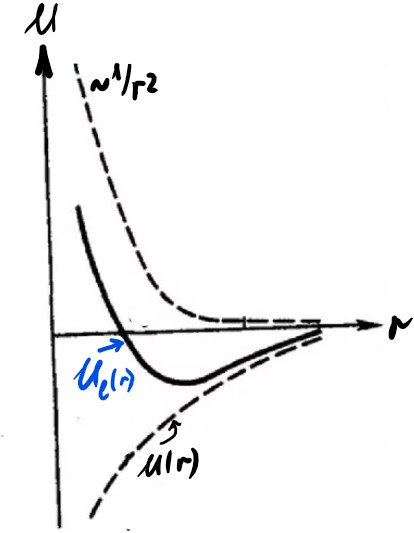
\includegraphics[width=1\linewidth]{pictures/27.1.jpg}
\caption{Измененный потенциал}
\end{wrapfigure}
\par Можем сократить сферические гармоники, получим
$$  \frac{1}{r^2}\frac{d}{d r} \left(r^2  \frac{d R}{d r} \right) -  \frac{l(l+1)}{r^2} R + \frac{2m}{\hbar^2} (E-U)R =0$$
\par Заменой $\chi = r R$ приводим к 
$$\chi^{\prime \prime}_{rr} + \left(\frac{2m}{\hbar^2} (E-U(r)) - \frac{l(l+1)}{r^2} \right) \chi =0$$

\par Задача определена на луче, требуем граничное условие $\chi(0) = 0 $, иначе получим расходимость в нуле для $R = \frac{\chi}{r}$.
\par Измененный потенциал $U_l (r) = U(r) + \frac{\hbar^2}{2m} \frac{l(l+1)}{r^2}$, где второе слагаемое описывает энергию вращения.
\par Уровни в потенциале нумеруются целыми числом $n_r$ - \textbf{квантовое радиальное число}. Кстати, полученные ранее числа $l$ и $m$ называются соответственно \textbf{квантовым азимутальным} и \textbf{квантовым магнитным числом}.
\par \begin{wrapfigure}[21]{l}{0.6\linewidth} 
\vspace{-2ex}
\centering
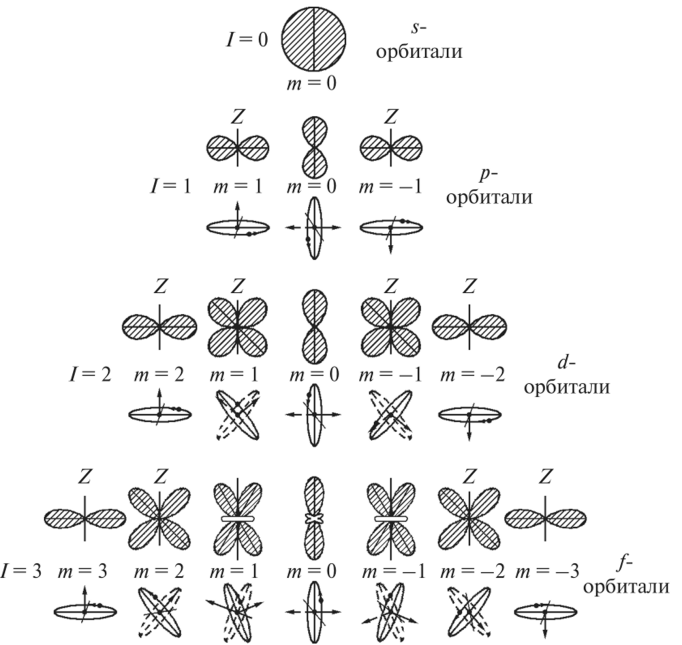
\includegraphics[width=1\linewidth]{pictures/27.2.png}
\caption{Атомные орбитали}
\end{wrapfigure}
\par Из атомной физики. Магнитное квантовое число m описывает ориентацию орбиталей в пространстве.
Для $l=0$ возможно только одно значение: $m=0$. Это значит, что s-орбиталь имеет только одну пространственную ориентацию.
Для $l=1$: $m=-1;0;+1$ - p-орбиталь имеет три пространственные ориентации.
Для $l=2$: $m=-2;-1;0;+1;+2$ - d-орбиталь имеет пять пространственных ориентаций.

